%%%%%%%%%%%%%%%%%%%%%%%%%%%%%%%%%%%%%%%%%%%%%%%%%%%%%%%%%%%%%%%%%%%%%%%%%%%%%%%%
\chapter{Постановка задачи и выбор пути решения}
%%%%%%%%%%%%%%%%%%%%%%%%%%%%%%%%%%%%%%%%%%%%%%%%%%%%%%%%%%%%%%%%%%%%%%%%%%%%%%%%

В данном разделе перечислены задачи, решаемые в ходе работы над данной магистерской диссертацией. Также в данном разделе указаны требования и ограничения, стоящие при выполнении поставленных задач.

%%%%%%%%%%%%%%%%%%%%%%%%%%%%%%%%%%%%%%%%%%%%%%%%%%%%%%%%%%%%%%%%%%%%%%%%%%%%%%%%
\section{Решаемые задачи}
%%%%%%%%%%%%%%%%%%%%%%%%%%%%%%%%%%%%%%%%%%%%%%%%%%%%%%%%%%%%%%%%%%%%%%%%%%%%%%%%

Ниже перечислены поставленные для данной магистерской диссертации задачи:
%
\begin{itemize*}
\item Разработать процедуру извлечения составляющих формальной спецификации библиотеки;
\item Разработать прототип инструмента автоматизированной генерации формальной спецификации библиотеки;
\item Проверить процедуру извлечения составляющих формальной спецификации библиотеки;
\end{itemize*}
%

%%%%%%%%%%%%%%%%%%%%%%%%%%%%%%%%%%%%%%%%%%%%%%%%%%%%%%%%%%%%%%%%%%%%%%%%%%%%%%%%
\section{Формулирование требований к разрабатываемой системе}
%%%%%%%%%%%%%%%%%%%%%%%%%%%%%%%%%%%%%%%%%%%%%%%%%%%%%%%%%%%%%%%%%%%%%%%%%%%%%%%%

%%%%%%%%%%%%%%%%%%%%%%%%%%%%%%%%%%%%%%%%
\subsection{Требования к процедуре извлечения составляющих формальной спецификации библиотеки}
%%%%%%%%%%%%%%%%%%%%%%%%%%%%%%%%%%%%%%%%

Процедура извлечения составляющих формальной спецификации библиотеки спецификации, должен быть рассчитан на использование с языком Java.

Процедура должна корректно обрабатывать код на языке Java 8.

Процедура должна иметь возможность работать как с исходным кодом(java-файлами) библиотеки, так и с jar-файлом библиотеки.

В процессе извлечения составляющих формальной спецификации библиотеки (или структуры спецификации) процедура должна анализировать исходный код функций.

Процедура извлечения структуры спецификации должна исключать все интерфейсы, которые присутствуют в библиотеке, а также те классы, которые не относятся к библиотеке.
Также необходимо исключать из анализа абстрактные классы и методы из библиотеки.

Процедура извлечения составляющих формальной спецификации должена обрабатывать все основные элементы программы, в которых используется библиотека: возвращаемое методом значение, аргументы метода, типы методов.

Процедура извлечения структуры спецификации должна в процессе работы формировать объекты, которые являются элементами LibSL спецификации, то есть результатом работы метода будут являться:
%
\begin{itemize*}
\item Заголовок библиотеки;
\item Описание подключаемых файлов или пакетов;
\item Описание псевдонимов типов;
\item Автомат, для каждого класса который есть в библиотеке;
\item Описание функций API (Application Programming Interface) библиотеки, для каждой публичной функции
\end{itemize*}
%
\nomenclature{API}{Application Programming Interface}

Дополнительно процедура извлечения спецификации необходимо извлекать из исходного текста библиотеки информацию о влиянии каждой функции на окружающую среду.

%%%%%%%%%%%%%%%%%%%%%%%%%%%%%%%%%%%%%%%%
\subsection{Требования к инструменту автоматизированной генерации спецификации}
%%%%%%%%%%%%%%%%%%%%%%%%%%%%%%%%%%%%%%%%

Инструмент должен реализовывать процедуру извлечения составляющих формальной спецификации библиотеки.
Разрабатываемый инструмент должен генерировать код на языке формальной спецификации LibSL.
Полученный код инструментом должен быть удобочитаемым для программиста. Например, имена переменных из сигнатуре функции библиотеки должны сохраняться, если это возможно.
Инструмент не должен допускать ошибок в сгенерированном коде спецификации.

Разрабатываемый инструмент должен быть кроссплатформенным и работать под управлением операционных систем

%%%%%%%%%%%%%%%%%%%%%%%%%%%%%%%%%%%%%%%%%%%%%%%%%%%%%%%%%%%%%%%%%%%%%%%%%%%%%%%%
\section{Анализ задач и выбор пути решения}
%%%%%%%%%%%%%%%%%%%%%%%%%%%%%%%%%%%%%%%%%%%%%%%%%%%%%%%%%%%%%%%%%%%%%%%%%%%%%%%%

Далее будет рассмотрен существующий вид статического анализа - анализ потока управления.
Ниже перечислены основные модели для анализа, которые можно выделить из такого вида статического анализа исходного кода или байт-кода библиотеки:
%
\begin{itemize*}
\item Анализ графа потока управления (CFG);
\item Анализ абстрактного синтаксического дерева (AST);
\end{itemize*}
%
\nomenclature{AST}{Abstract Syntax Tree}
\nomenclature{CFG}{Control Flow Graph}

Процедура будет получать на вход исходный код программы и далее представлять его в виде удобной модели программы для проведения анализа.
Модели программы обеспечивают доступ ко всем объектам программного кода и их атрибутам. Также поддерживают эффективный поиск объектов и снимают сложность разработки методов статического анализа.

%%%%%%%%%%%%%%%%%%%%%%%%%%%%%%%%%%%%%%%%
\subsection{Анализ графа потока управления}
%%%%%%%%%%%%%%%%%%%%%%%%%%%%%%%%%%%%%%%%

Граф потока управления представляется в виде ориентированного графа. В нем сохраняется вся необходимая информация о конструкциях программы и переходах между ними.

При построение CFG также учитываются:
%
\begin{itemize*}
\item Безусловные переходы;
\item Ветвления;
\item Циклы;
\item Вызовы функций;
\item Исключения;
\end{itemize*}
%

На Рис.~\ref{fig:cfg_example_1} представлен пример графа потока управления.

\begin{figure}[htbp]
\centering
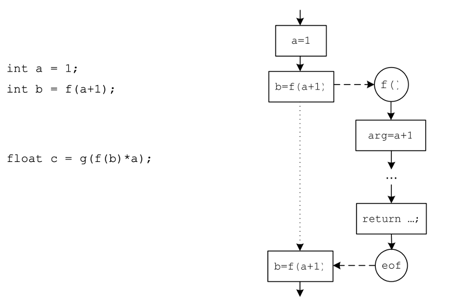
\includegraphics[width=\textwidth]{fig/cfg_example_1.png}
\caption{Пример CFG}%
\label{fig:cfg_example_1}
\end{figure}

%%%%%%%%%%%%%%%%%%%%%%%%%%%%%%%%%%%%%%%%
\subsection{Анализ абстрактного синтаксического дерева}
%%%%%%%%%%%%%%%%%%%%%%%%%%%%%%%%%%%%%%%%

На Рис.~\ref{fig:ast_example_1} представлено абстрактное синтаксическое дерево, оно представляет собой древовидное представление структуры исходного кода, где листья представляются в качестве константы или переменной, а внутренние узлы - операторы.

\begin{figure}[htbp]
\centering
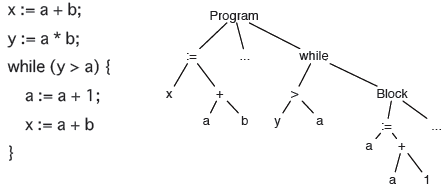
\includegraphics[width=\textwidth]{fig/ast_example_1.png}
\caption{Пример AST}%
\label{fig:ast_example_1}
\end{figure}

AST используют как в разработке программ, так и в анализе программ.
AST лучше всего представляет синтаксическую структуру исходного кода. AST независим от конкретного синтаксиса для идентификаторов, операторов, условий или утверждений базового языка программирования.

Представление AST можно считать не только промежуточным, а также использовать его для различных оптимизаций. Преимуществом использования абстрактного синтаксического дерева является более высокий уровень абстракции по сравнению с исходным кодом программы.

%%%%%%%%%%%%%%%%%%%%%%%%%%%%%%%%%%%%%%%%%%%%%%%%%%%%%%%%%%%%%%%%%%%%%%%%%%%%%%%%
\section{Выводы}
%%%%%%%%%%%%%%%%%%%%%%%%%%%%%%%%%%%%%%%%%%%%%%%%%%%%%%%%%%%%%%%%%%%%%%%%%%%%%%%%

В данном разделе были сформулированы задачи, которые актуальны для этой магистерской работы. Были определены требования к разрабатываемой системе автоматизации генерации формальной спецификации библиотек.
В ходе анализа задачи было принято решение об использовании статического анализа кода, а именно метода анализа абстрактного синтаксического дерева при проектировании процедуры извлечения составляющих формальной спецификации библиотеки.
Выбор был сделан для упрощения, а также из-за нехватки времени. Это даст нам более грубый результат, при более простом пути решения.